%!TEX root = main.tex
\section{Introduction}

%\section{History of Non-Photorealistic Rendering}
Over the last 30 years, computer graphics researchers have tried to achieve photorealistic images by using computer programs \cite{strothotte02}. Ivan Sutherland was one of the pioneers in creating computer generated photorealistic images, working in the early 1960s. Photorealistic computer graphics is essentially an attempt to imitate real life pictures that would be normally taken by using another tools such as camera. Such attempts usually occurs in 3 dimensional (3D) computer graphics, which in most cases, try to render the 3D model as realistically as possible. At the early stage of computer graphics research, these attempts has been failed in many cases, especially on the attempts to imitate human appearance. Recent research, however, has started to show more believable lifelike human facial animation \cite{emily08}. More recently, instead of producing results that look like real life objects, researchers have tried to produce more cartoon-looking or hand-drawn images; this technique is known as Non-photorealistic Rendering.

Non-Photorealistic Rendering (NPR) is a process which uses a computer program to produce non-photorealistic renditions \cite{strothotte02}, such as sketch illustration, oil painting, watercolor-painting, etc. While using photorealistic images or even real photographs may deliver accurate information to the viewers, they also possess some weaknesses, which can be surpassed by hand-drawn images. In some cases, hand-drawn images can actually delivers more information because they can allocate more focus on a certain aspect of a picture while ignoring unimportant ones. This way, the viewers will focus their attention on what the picture tried to convey. These kinds of images can be found in technical illustrations, for example in user manual of some electronic devices, or can also be found in medical illustrations.

Hand-drawn images can also be used to show the preliminary stage of a design in design phase period. For example, in architectural design \cite{schumann96},  architects usually use pencil sketch drawings to show a draft of a design. The viewer can get the feeling of this preliminary stage better when seeing a hand-drawn pencil sketch image compared to a photorealistic image.

Another benefit of using hand-drawn images is to give aesthetic feeling to an image. Images, such as paintings created by an artist, usually have aesthetic values that can stimulate certain emotions in humans. While the paintings themselves might not look as realistic as a photograph, they usually can stimulate senses and emotions in the people who see it.

The goal of NPR is to try to achieve the same benefits of using hand-drawn images in cases when an actual hand-drawn image is very difficult or impossible to create. The source of image generation on NPR can come from either 3 dimensional model or photographs taken by camera.

Since the first time NPR was introduced, there have been many researches to work on the topic. Many of them have created techniques of imitating different styles of hand-drawing period. For example: sketch rendering \cite{strothotte94}, pen-and-ink illustration \cite{winkenbach94},\cite{salisbury94}, stipple drawing \cite{secord02},\cite{deussen00}, painterly effect \cite{litwinowicz97},\cite{hertzmann98},\cite{hays04}, and line drawing \cite{decarlo03}, \cite{sousa03},\cite{kang07}.

%\chapter{Background}

\section{Line Drawing} 
Line drawing is a drawing style that is commonly used to create illustration, such as technical illustrations and medical illustrations, caricature drawings, sketch drawings, etc. Line drawing uses straight or curved lines to form an image. Some techniques, such as stippling or hatching, can be used to show different levels of shade. Line drawing has become one of the primary branches of NPR. Techniques have been improving in creating more believable results compared to line drawing illustration made by an artist. Line drawing in NPR can be divided into two categories based on the source of the image, which can be a 3D object or a 2D object. Many works have been introduced on line drawing based on 3D object \cite{decarlo03}, \cite{sousa03}. Creating line drawing images from 3D models is relatively easier compared to 2D objects. In 3D models, the edge can be easily identified because all the information is stored in a straightforward manner, while in 2D objects, such as in photographs, information about edges are more difficult to extract and require extra steps and complicated methods to achieve a good result.

Most work in line drawing in NPR is based on edge detection or image segmentation techniques. The difference between edge detection and line drawing is that edge detection is more focused on how to extract edges from a picture without considering the aesthetic aspect of how the lines (edges) are compounded. While line drawing in NPR is also trying to extract edges from pictures and form lines, it attempts to create a more artistic result, as if the image were created by human artist. Some aspects that need to be considered to produce artistic results are: the structures of the lines and the use of stylistic edges. There are many methods to do edge detection, two examples of them are Canny's method \cite{canny86}, and Marr-Hildreth's method \cite{marr-hildreth80}, which became the base for Difference-of-Gaussian (DoG) filter and used by Gooch et al. in their facial illustration system to create some artistic line drawing.

\section{Difference of Gaussian (DoG)} 
Gooch et al. in their facial illustration system \cite{gooch04} were able to create some artistic results. They were able generate a caricature of a human face based on a photograph. Their method uses DoG filter, which was based on Marr-Hildreth's edge detection.

The basic idea of DoG is to apply 2 Gaussian filters with different blur levels ($\sigma$). The second Gaussian filter uses a bigger blur radius to create blurrier image compared to the image produced by the first Gaussian filter. The Area close to edges will have more changes compared to area far from edges if applied to Gaussian filter with different blur level. The difference of intensity of each pixel of these two blurred images will be use by DoG to obtain edges, as shown in Figure ~\ref{fig:DoG_sample1}.

\begin{figure}[H]
\centering
	\subfigure[Input image] {
		\includegraphics[width=1.8in]{pictures/beach_rock_boat/image.eps}
	}
	\subfigure[Gaussian with $\sigma = 1.0$] {
		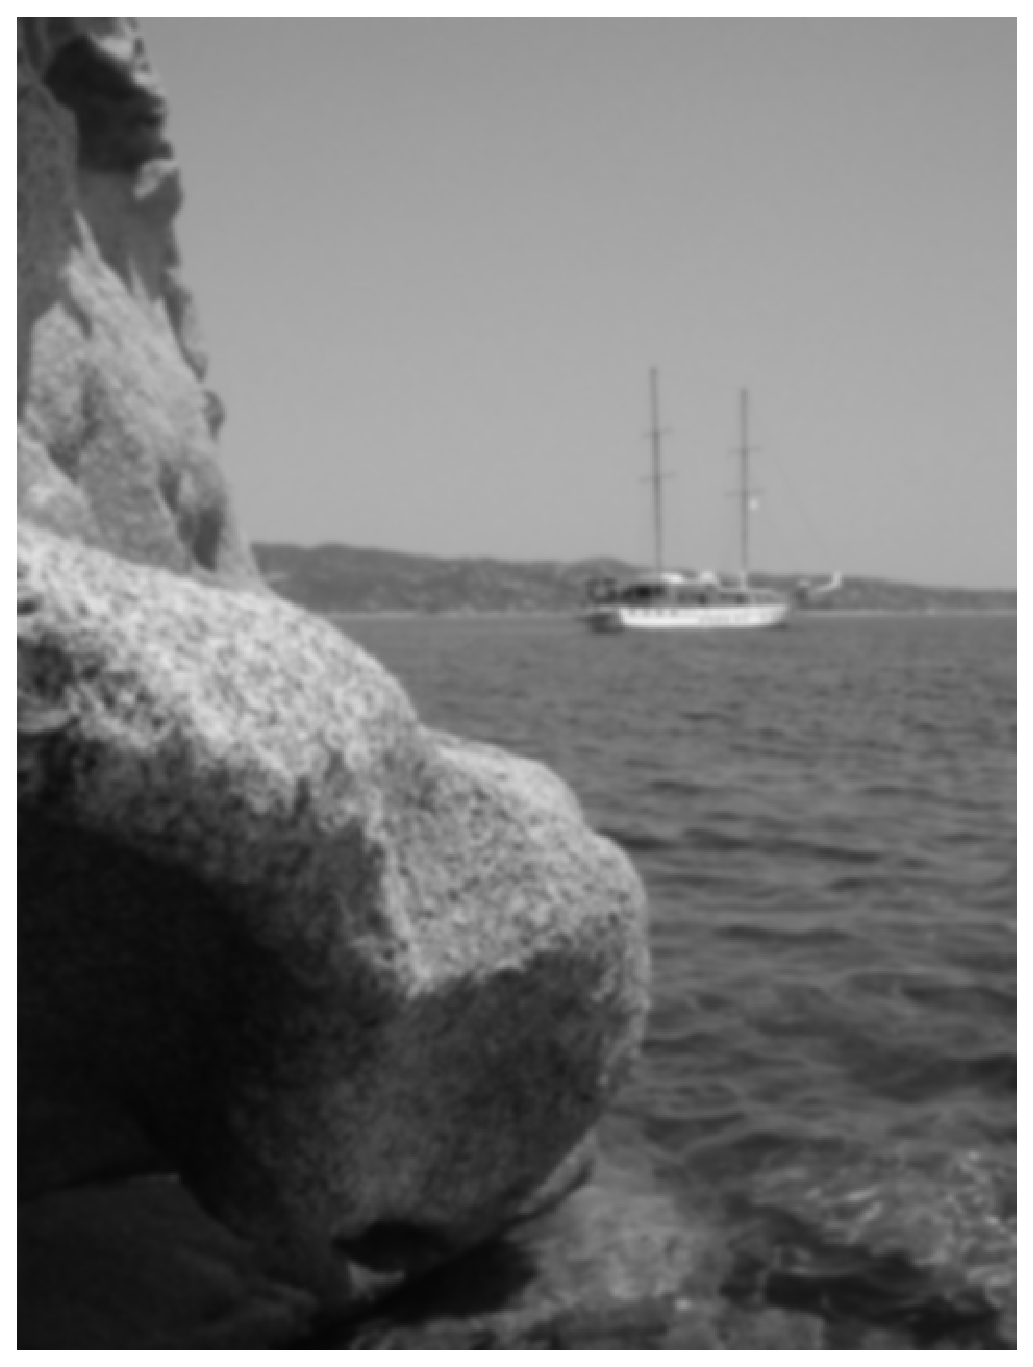
\includegraphics[width=1.8in]{pictures/beach_rock_boat/gaussian1.eps}
	}
	\subfigure[Gaussian with $\sigma = 1.6$] {
		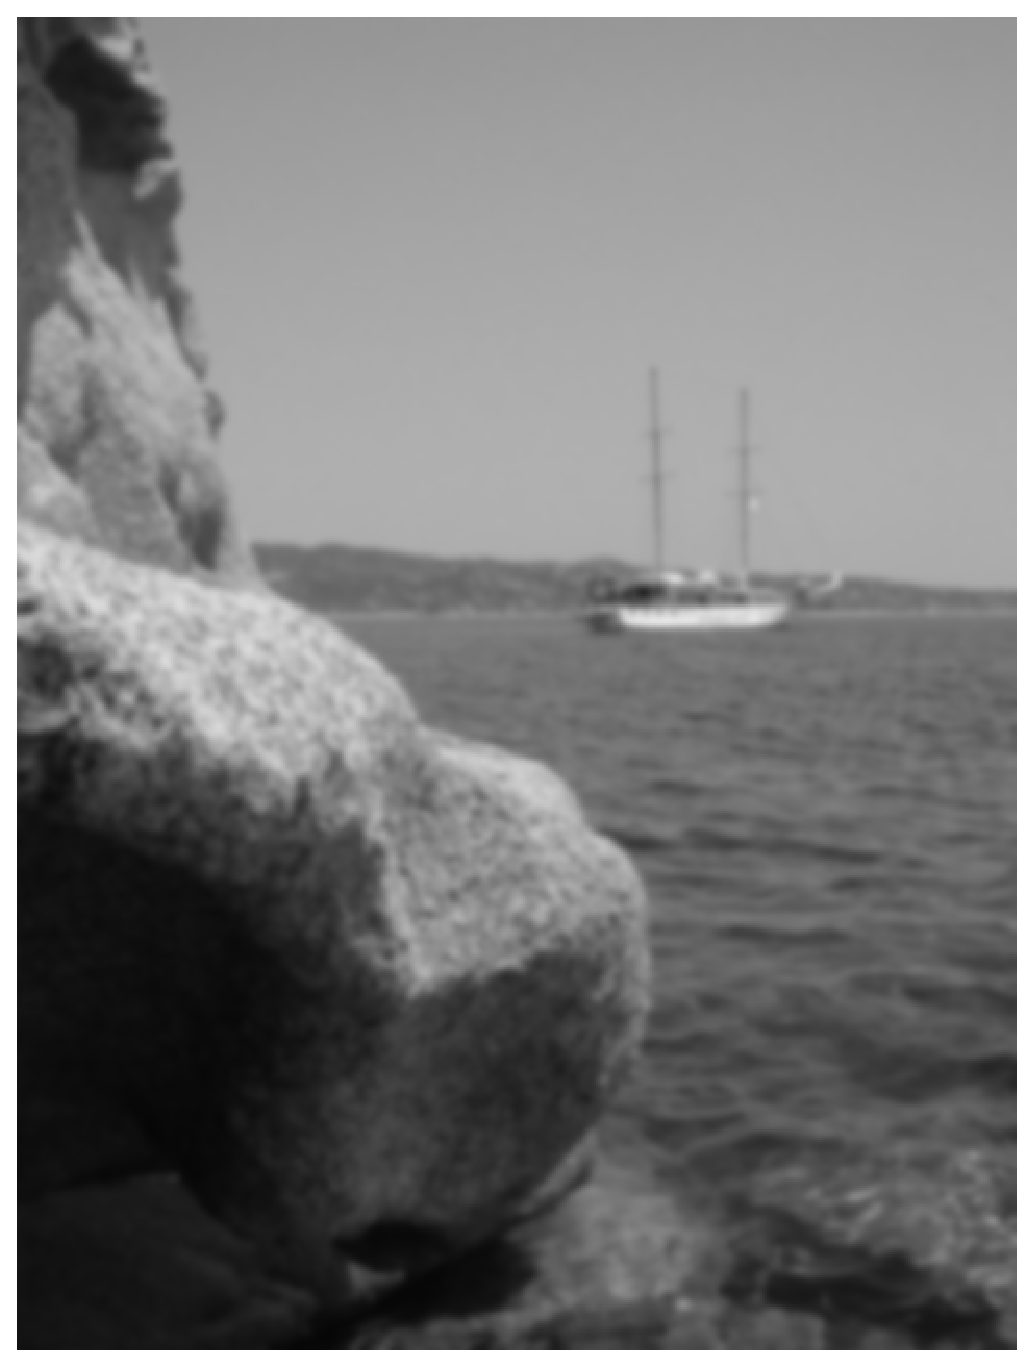
\includegraphics[width=1.8in]{pictures/beach_rock_boat/gaussian2.eps}
	}
\caption{Sample of gaussian filter}
\label{fig:DoG_sample1}
\end{figure}

%Gaussian Function
The Gaussian function used in DoG is formulated as the following 1-dimensional Gaussian function:
\begin{equation}
	G(i, \sigma) = \frac{1}{\sqrt{2\pi\sigma}}e^{-\frac{i^2}{2\sigma^2}}
\end{equation}
where $\sigma$ is the blur level. $G(i, \sigma)$ is used as weight factor on how intensity of each pixel and its neighbor will influence intensity of the output, thus creating a blur image. 

\begin{figure}[H]
	\centering
	\subfigure[DoG Kernel] {
		\psset{unit=1.5}
		\begin{pspicture}(-1.5,-1.5)(1.5,1.5)
		\psaxes[labels=none, ticks=none,axesstyle=frame]{}(0,0)(-1,-1)(1,1)
		\rput(-1.3, 0){\textit{-T}}
		\rput(1.3, 0){\textit{T}}
		\rput(0, -1.3, 0){\textit{-S}}
		\rput(0, 1.3, 0){\textit{S}}
		\pscurve{<-}(0.5,0.05)(0.7,0.4)(1.3,0.5)
		\pscurve{<-}(0.05,0.5)(0.4,0.7)(0.5, 1.3)
		\rput(1.5,0.5){$l_{x}$}
		\rput(0.5,1.5){$l_{y}$}
		\rput(0.15,0.15){$\mbox{x}$}
		\psdot[dotstyle=*, dotsize=4pt](0,0)
		\end{pspicture}
	}
	\subfigure[Gaussian components for DoG] {
		\psset{unit=1.5}
		\begin{pspicture}(-2,-0.5)(2,2) 
		\psaxes[labels=none,ticks=none]{}(0,0)(-1.5,0)(1.5,1.5)
		\rput(-1,-0.2){\textit{-T}}
		\rput(1,-0.2){\textit{T}}
		\rput(0,-0.2){0}
		\psGauss[linecolor=red, linewidth=1pt, sigma=0.5]{-1.5}{1.5}
		\psGauss[linecolor=blue, linewidth=1pt, sigma=0.3125]{-1}{1}
		\psline{->}(0.5,1.7)(0.2,1.2)
		\rput(0.6,1.8){$G_{\sigma_{c}}$}
		\psline{->}(1.2,0.7)(0.9,0.2)
		\rput(1.3,0.8){$G_{\sigma_{s}}$}
		\end{pspicture}
	}
	\caption{Difference of Gaussian filtering}\label{fig:image}
\end{figure}

This weight factor applied with $\sigma_{c}$ for each intensity of pixels along line $l_{x}$ started from $-T$ to $T$:
\begin{equation}
	f(t, \sigma)=\int_{-T}^{T}G(t, \sigma)I(l_{x}(t))\,dt
\end{equation}
and using the value from $f(t, \sigma)$, we use 
We then apply the same function along line $l_{y}$ starting from -S to S, and repeat this steps for every pixel on input image to produce a blurred image.
\begin{equation}
	F(\mbox{x}, \sigma)=
		\int_{-S}^{S}G(s, \sigma)f(l_{y}(s), \sigma)\,ds
\end{equation}
The same procedure with $\sigma_{s} = 1.6\sigma_{c}$ is then applied to the same input image, producing another blurred image.
From these 2 output images, we then able to calculate differences of each pixel's intensity, and capture edges of the input image (Figure ~\ref{fig:DoG}).

\begin{equation}
	H_{d}(\mbox{x}) = F(\mbox{x},\sigma_{c}) - \rho\cdot F(\mbox{x},\sigma_{s})
\end{equation}

\begin{figure}[H]
	\centering
	\subfigure[Rock and Boat]{
	\includegraphics[width=2in]{pictures/beach_rock_boat/dog.eps}
	}
	\subfigure[Baboon]{
	\includegraphics[width=2.5in]{pictures/baboon/dog.eps}
	}
	\caption{Difference-of-Gaussian}\label{fig:DoG}
\end{figure}

\section{Flow-based Difference of Gaussian} 
Difference-of-gaussian (DoG) method has the nature of isotropic because the filter moves to every direction in order to calculate the differences. This nature, when applied to images with anisotropic characteristic, will create a lot of discontinuity lines because it failed to follow the direction alongside the edges. So, instead of moving to every direction, Kang et al. are suggesting to incorporate direction guide to the filter that follows the direction of edges \cite{kang07}.

To create the direction guidance for DoG filter, Kang et al., use the information from edge flow, which is where an area of image has high contrast of intensity level, and run the DoG filter perpendicular to the edge flow direction. By providing guide for the filter direction, Kang et al., were able to produced more coherent and continues line drawing \cite{kang07}. 


\subsection{Edge Tangent Flow} 
Kang et al., technique in creating line drawing required two steps. First step is to generate edge tangent flow that will provide direction to run DoG filter. To create edge tangent flow from input image $ I(\mbox{x}) $, where $ \mbox{x} = (x,y)$ denotes a pixel at coordinate $(x,y)$, Kang et al., use edge tangent $\mbox{t}(\mbox{x}) $ as a vector perpendicular to the image gradient $ g(\mbox{x}) = \nabla I(\mbox{x})$, and called it Edge Tangent Flow (ETF). 

They presented a technique to construct ETF by using kernel-based nonlinear smoothing of vector field. The ETF construction filter is as follows:
\begin{equation}
	\mbox{t} ^{new}(\mbox{x} ) = \frac{1}{k} \sum_{\mathrm{x}' \in \Omega (\mathrm{x})} \phi (\mbox{x},\mbox{x}') \mbox{t} ^{cur} (\mbox{y}) w_s(\mbox{x},\mbox{x}') w_m(\mbox{x},\mbox{x}') w_d(\mbox{x},\mbox{x}')
\end{equation}

where $ k $ is the vector normalizing term and $\Omega(\mbox{x})$ is the neighbor of $\mbox{x}$. ETF function uses 3 weight function, the first one is $w_s$, a \textit{spatial weight function}, which uses radially-symmetrical box filter with radius of $r$, where $r$ is the radius of kernel $\Omega$. The \textit{spatial weight  function} $w_s$ is defined as following:

\newcommand{\norm}[1]{\left\| #1 \right\|}
\begin{equation}
	w_s(\mbox{x}, \mbox{x}') = 
	\left\{
		\begin{array}{ll}
			1&\mbox{ if }\norm{\mbox{x} - \mbox{x}'} < r
			\\0&\mbox{ otherwise }
		\end{array}
	\right.
\end{equation}

The second weight function is $w_m$, a \textit{magnitude weight function}, which is defined as following:
\begin{equation}
	w_m(\mbox{x}, \mbox{x}') = \frac{1}{2} (1 + \textrm{tanh}[\eta \cdot (\hat{g}(\mbox{x}') - \hat{g}(\mbox{x}) )])
\end{equation}
where $\hat{g}(\mbox{x})$ and $\hat{g}(\mbox{x}')$ denotes normalized gradient magnitude at $\mbox{x}$ and $\mbox{x}'$ respectively. Variable $\eta$ is the weight variable that determine how the neighboring pixel $\mbox{x}'$ with gradient value higher than gradient value of $\mbox{x}$ will influence the edge tangent $\mbox{t}(\mbox{x})$. 

The third weight function is the direction weight function $w_d$, which is defined as following:
\begin{equation}
	w_d(\mbox{x}, \mbox{x}') = |\mbox{t}^{cur}(\mbox{x})\cdot \mbox{t}^{cur}(\mbox{x}')|
\end{equation}
where $\mbox{t}^{cur}(\mbox{x})$ and $\mbox{t}^{cur}(\mbox{x})$ denote the current normalized tangent vector at $\mbox{x}$ and $\mbox{x}'$ respectively. This function is using a dot product between tangent vectors at a particular location with its neighbors'. The cross product produce a high weight value for vectors that are closely aligned (where angle between two vectors ($\theta$) is close to $0^{\circ}$ or $180^{\circ}$) and produce a low weight value for vectors that are perpendicular to each other (where angle between two vector ($\theta$) is close to $90^{\circ}$).

The last function is used to reverse the direction of $\mbox{t}^{cur}(\mbox{x}')$ before smoothing when angle between vectors ($\theta$) is bigger than $90^{\circ}$ (dot product between two vectors is < 0):
\begin{equation}
	\phi(\mbox{x}, \mbox{x}') = 
	\left\{
		\begin{array}{ll}
			1&\mbox{ if }\mbox{t}^{cur}(\mbox{x})\cdot \mbox{t}^{cur}(\mbox{x}') > 0
			\\-1&\mbox{ otherwise }
		\end{array}
	\right.
\end{equation}

As shown in the function, $\mbox{t}^{new}(\mbox{x})$ is achieved from applying all functions to $t^{cur}(\mbox{x})$, and initially, $\mbox{t}^{\circ}(\mbox{x})$ is achieved from normalized vector perpendicular to gradient $g(\mbox{x})$ in gradient map of the input image $I$. ETF is constructed by iteratively apply $\mbox{t}(\mbox{x})$ function several times (in this experiment, we applied 2 or 3 times).


\subsection{Flow-based DoG}
%\begin{equation}
%	G_{\sigma}(x) = \frac{1}{\sqrt{2\pi\sigma}}e^{-\frac{x^2}{2\sigma^2}}
%\end{equation}
After constructing ETF, the next step will be applying anisotropic DoG with edge flow information from ETF to guide its direction. We build kernel whose shape is based on local flow from ETF, and apply DoG on this kernel. Examples of kernel is shown in Figure ~\ref{fig:FDoG_kernel}. Line $c_{x}$ is a line that follows direction of flow from ETF, and line $l_{s}$ is a line tangent to line $c_{x}$. 
\begin{figure}[H]
	\centering
	\subfigure[FDoG Kernel] {
		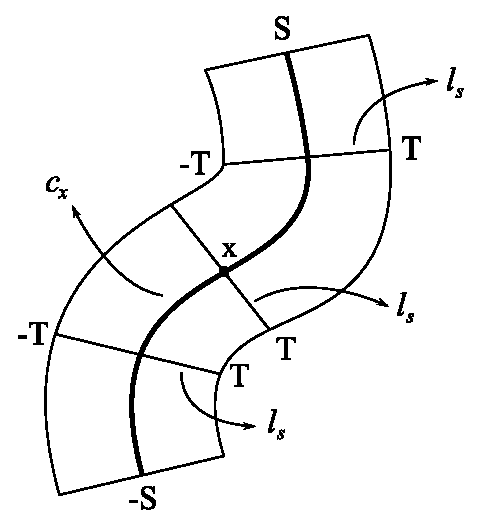
\includegraphics[width=1.5in]{pictures/fdog_kernel.eps}
	}
	\subfigure[Gaussian components for DoG] {
		\psset{unit=1.5}
		\begin{pspicture}(-2,-0.5)(2,2) 
			\psaxes[labels=none,ticks=none]{}(0,0)(-1.5,0)(1.5,1.5)
			\rput(-1,-0.2){\textit{-T}}
			\rput(1,-0.2){\textit{T}}
			\rput(0,-0.2){0}
			\psGauss[linecolor=red, linewidth=1pt, sigma=0.5]{-1.5}{1.5}
			\psGauss[linecolor=blue, linewidth=1pt, sigma=0.3125]{-1}{1}
			\psline{->}(0.5,1.7)(0.2,1.2)
			\rput(0.6,1.8){$G_{\sigma_{c}}$}
			\psline{->}(1.2,0.7)(0.9,0.2)
			\rput(1.3,0.8){$G_{\sigma_{s}}$}
		\end{pspicture}
	}	
	\caption{Flow-based DoG Kernel}\label{fig:FDoG_kernel}
\end{figure}

We first apply 1 dimensional filter $f(t)$ along the line $l_{s}$:
\begin{equation}
	F(s) = \int_{-T}^{T} I(l_s(t))f(t)\,dt
\end{equation}
where $l_s(t)$ denotes a pixel on the line $l_s$ at parameter $t$, and $I(l_s(t))$ is intensity level of the pixel. Function $f(t)$ is the same DoG function from previous chapter that use 2 gaussian filters with difference $\sigma$ and then calculate differences from 2 output values. 
\begin{equation}
	f(t) = G_{\sigma_{c}}(t)-\rho \cdot G_{\sigma_{s}}(t)
\end{equation}
$\rho$ value control the level of noise detected, and in this experiment, we use value of 0.99.

After applying filter $f(t)$ to each pixel, we then apply filter $F(t)$ along line $c_{x}$ from $-S$ to $S$ on FDoG kernel. 
\begin{equation}
	H_{f}(\mbox{x}) = \int_{-S}^{S} G_{\sigma_{m}}(s)F(s)\,ds
\end{equation}
where $G_{\sigma_{m}}$ is another gaussian function that will become weight factor for each responses according to $s$. As shown in Figure ~\ref{fig:FDoG}, image from FDoG () has continuous lines and less noise compared to DoG.

\begin{figure}[H]
	\centering
	\subfigure[Input image]{
	\includegraphics[width=2in]{pictures/window/image.eps}
	}
	\subfigure[DoG]{
		\setlength\fboxsep{0pt}
		\setlength\fboxrule{0.5pt}
		\label{fig:DoG_sample}
		\fbox{\includegraphics[width=2in]{pictures/window/dog.eps}}
	}
	\subfigure[FDoG]{
		\setlength\fboxsep{0pt}
		\setlength\fboxrule{0.5pt}
		\label{fig:FDoG_sample}
		\fbox{\includegraphics[width=2in]{pictures/window/cld.eps}}
	}
	\caption{Difference-of-Gaussian}\label{fig:FDoG}	
\end{figure}


\chapter{Hybrid}
Base on the output, images created by FDoG contained more coherent and continuous lines compared to images created by DoG. The directional kernel used in FDoG was proven to be able to create lines on anisotropic images, and created good line drawing images. One major drawback of FDoG is it cannot capture all the detail on images with isotropic characteristic. Example on Figure ~\ref{fig:FDoGWeakness} shows that FDoG failed to capture the details of grained textures, furthermore creating lines in area where it is not supposed to be. While DoG can easily cope with this flaw, it still cannot outmatch FDoG in cases of anisotropic images. These two different characteristics of FDoG and DoG on handling isotropic and anisotropic images bring us to the idea of combining to method in order to achieve optimal results in both cases.

\begin{figure}[H]
	\centering
	\subfigure[Input Image] {
		\includegraphics[width=1.5in]{pictures/texture/image.eps}
	}
	\subfigure[DoG] {
		\includegraphics[width=1.5in]{pictures/texture/dog.eps}
	}
	\subfigure[FDoG] {
		\includegraphics[width=1.5in]{pictures/texture/cld.eps}
	}
	\caption{Weakness of FDoG}\label{fig:FDoGWeakness}
\end{figure}

\section{Combining FDoG with DoG}
The simple method to combine DoG and FDoG is by applying linear combination of FDoG and DoG functions, and called it Hybrid DoG:
\begin{equation}
	H_{h}(\mbox{x}) = \lambda H_{f}(\mbox{x}) + (1 - \lambda) H_{d}(\mbox{x})
\end{equation}
Value of $\Lambda$ will determine the closeness of the output to FDoG or DoG, when the value of $\Lambda$ approaches 0, it will produce output that similar to DoG, and will produce output similar to FDoG when it approaches 1. 

With this variable $\lambda$, we can control the behavior of the filter according to the character of input images. Use value of $\lambda$ close to 0 for input images with majority of isotropic images, and use value of $\lambda$ close to 1 for anisotropic images. For images with both isotropic and anisotropic characteristic, based on our experiment, values of 0.5 for $\lambda$ will produce good results for most of the images.

\chapter{Adaptive-DoG Technique}
Another method to combine DoG and FDoG is to adaptively apply the right filter for different area depending on their characteristic. Area with isotropic textures will use DoG to retain the texture, while area with anisotropic detail will use FDoG to create more coherent lines and low noise details. To be able to adaptively apply the right filter, we first need to be able to distinguish between isotropic and anisotropic segment. Belongie et al., \cite{belongie98} in their paper use polarity to segment the image based on texture type. We simplify the technique used by Belongie et al.

\section{Image Segmentation} 
Polarity is calculated by comparing the gradient's direction of a pixel to its neighbor's gradients. Area with similar gradient vector direction considered as high polarity area, while area with non-uniform gradient vector direction is considered as low polarity area. Non-uniform gradient vector direction is can be found in isotropic area the gradients in this area scattered. Anisotropic area will have more uniform and similar direction, although it may also has have gradients facing opposite to each other as we can see on area with stripe texture. Using this behavior, we can distinguish between isotropic and anisotropic area by determining polarity of each pixel. One exception that need to be considered is isotropic area with low gradient magnitude should be considered as isotropic segment since this area should be applied with FDoG filter to minimize noise.

To calculate polarity, we use a function $S$ which will be applied to pixel location $\mbox{x}$:
\begin{equation}
	S(\mbox{x})=\frac{\sum\limits_{\mathrm{x}' \in \Omega (\mathrm{x})}\left|\,g(\mbox{x}) \cdot g(\mbox{x})'\,|\right.}
		{\left|\,\Omega(\mathrm{x})\,|\right.}
\end{equation}
where $\Omega(\mbox{x})$ is the neighborhood of pixel $\mbox{x}$ and pixel $\mbox{x}'$ is element of $\Omega(\mbox{c})$. We use absolute value for dot product between two gradient vector because we consider vectors with opposite direction in the same segment. The sum of dot product is then divided by ${\left|\,\Omega(\mathrm{x})\,|\right.}$, the total number of pixels in the neighborhood, to get the average.

Next step will be segmenting the image using the polarity measured on previous step:
%binarize
\begin{equation}
	P(\mbox{x})=
		\left\{
			\begin{array}{ll}
				0&\mbox{ if }S(\mbox{x}) >= \alpha \;\mbox{or}\; \left|g(\mbox{x})|\right. < \beta
				\\
				1&\mbox{ otherwise }
			\end{array}
		\right.
\end{equation}
We use a threshold $\alpha$ as a cut point for polarity level, and in our experiment, we use $\alpha = 0.875$. Area with polarity above the threshold will be considered as anisotropic segment (labeled with $1$). For isotropic segment (labeled with $0$), since we also consider isotropic area with low gradient magnitude as anisotropic segment, we also need to consider the gradient magnitude. Variable $\beta$ is threshold for gradient magnitude at pixel $\mbox{x}$ and we use $\beta = 0.1$ in our experiment. 
\begin{figure}[H]
	\centering
	\subfigure[Input image]{
		\label{fig:Polarity_input}
		\includegraphics[width=2.5in]{pictures/coffeebeans/image.eps}
	}
	\subfigure[Polarity-based image segment; white indicates isotropic area, black indicates anisotropic area, and gray indicates area with low gradient magnitude]{
		\label{fig:Polarity_sample1}
		\includegraphics[width=2.5in]{pictures/coffeebeans/polarity.eps}
	}
	\caption{Image Segmentation}
\end{figure}

\section{Adaptive-DoG}

Once we obtain the image segment, the next step to adaptively apply hybrid DoG will be straightforward. Provided the characteristic of each area, we are now able to determine the proper filter for different area just by using label from the image segment. 
\begin{equation}
	H_{a}(\mbox{x})=
		\left\{
			\begin{array}{ll}
				H_{d}(\mbox{x})&\mbox{ if }P(\mbox{x}) = 0
				\\
				H_{d}(\mbox{x})&\mbox{ otherwise }
			\end{array}
		\right.
\end{equation}
Segment labeled with $0$ is isotropic area and use DoG filter $H_{d}$, while anisotropic area labeled with $1$ is applied with FDoG filter $H_{f}$. 

\chapter{Results}
The results of this adaptive technique have coherent lines similar to lines in FDoG, while still maintaining the details in coarser area. The lines as shown in figure ~\ref{fig:Adaptive_sample} around the shoe area have similar shape with lines from FDoG, while the surrounding textures still maintain its original shape.

\begin{figure}[H]
	\centering
	\subfigure[Input Image]{
		\label{fig:Adaptive_input}
		\includegraphics[width=2.5in]{pictures/shoes/image.eps}
	}
	\subfigure[Adaptive-DoG]{
		\setlength\fboxsep{0pt}
		\setlength\fboxrule{0.5pt}
		\label{fig:Adaptive_sample}
		\fbox{\includegraphics[width=2.5in]{pictures/shoes/adaptive.eps}}
	}
	\caption{Adaptive-DoG}\label{fig:Adaptive_DoG}
\end{figure}

%\section{Comparison with DoG and FDoG} 
\begin{figure}[H]
	\centering
	\subfigure[Input Image]{
		\setlength\fboxsep{0pt}
		\setlength\fboxrule{0.5pt}
		\fbox{\includegraphics[width=2.4in]{pictures/beach_rock_boat/image.eps}}
	}	
	\subfigure[Polarity Segment]{
		\setlength\fboxsep{0pt}
		\setlength\fboxrule{0.5pt}
		\fbox{\includegraphics[width=2.4in]{pictures/beach_rock_boat/polarity.eps}}
	}
	\subfigure[Adaptive-DoG]{
		\setlength\fboxsep{0pt}
		\setlength\fboxrule{0.5pt}
		\fbox{\includegraphics[width=2.4in]{pictures/beach_rock_boat/adaptive.eps}}
	}
	\caption{Boat and Rock}\label{fig:Compare1}
\end{figure}

\begin{figure}[H]
	\centering
	\subfigure[Input Image]{
		\setlength\fboxsep{0pt}
		\setlength\fboxrule{0.5pt}
		\fbox{\includegraphics[width=2.4in]{pictures/boat_in_sand/image.eps}}
	}	
	\subfigure[DoG]{
		\setlength\fboxsep{0pt}
		\setlength\fboxrule{0.5pt}
		\fbox{\includegraphics[width=2.4in]{pictures/boat_in_sand/dog.eps}}
	}
	\subfigure[FDoG]{
		\setlength\fboxsep{0pt}
		\setlength\fboxrule{0.5pt}
		\fbox{\includegraphics[width=2.4in]{pictures/boat_in_sand/cld.eps}}
	}
	\subfigure[Adaptive-DoG]{
		\setlength\fboxsep{0pt}
		\setlength\fboxrule{0.5pt}
		\fbox{\includegraphics[width=2.4in]{pictures/boat_in_sand/adaptive.eps}}
	}
	\caption{A Boat in Beach}\label{fig:Compare2}
\end{figure}

\begin{figure}[H]
	\centering
	\subfigure[Input Image]{
		\setlength\fboxsep{0pt}
		\setlength\fboxrule{0.5pt}		
		\fbox{\includegraphics[width=2.4in]{pictures/sand_dollar/image.eps}}
	}	
	\subfigure[DoG]{
		\setlength\fboxsep{0pt}
		\setlength\fboxrule{0.5pt}
		\fbox{\includegraphics[width=2.4in]{pictures/sand_dollar/dog.eps}}
	}
	\subfigure[FDoG]{
		\setlength\fboxsep{0pt}
		\setlength\fboxrule{0.5pt}
		\fbox{\includegraphics[width=2.4in]{pictures/sand_dollar/cld.eps}}
	}
	\subfigure[Adaptive-DoG]{
		\setlength\fboxsep{0pt}
		\setlength\fboxrule{0.5pt}
		\fbox{\includegraphics[width=2.4in]{pictures/sand_dollar/adaptive.eps}}
	}
	\caption{Sand Dollar}\label{fig:Compare3}
\end{figure}

\begin{figure}[H]
	\centering
	\subfigure[Input Image]{
		\setlength\fboxsep{0pt}
		\setlength\fboxrule{0.5pt}
		\fbox{\includegraphics[width=2.4in]{pictures/boat_in_sf/image.eps}}
	}	
	\subfigure[DoG]{
		\setlength\fboxsep{0pt}
		\setlength\fboxrule{0.5pt}
		\fbox{\includegraphics[width=2.4in]{pictures/boat_in_sf/dog.eps}}
	}
	\subfigure[FDoG]{
		\setlength\fboxsep{0pt}
		\setlength\fboxrule{0.5pt}
		\fbox{\includegraphics[width=2.4in]{pictures/boat_in_sf/cld.eps}}
	}
	\subfigure[Adaptive-DoG]{
		\setlength\fboxsep{0pt}
		\setlength\fboxrule{0.5pt}
		\fbox{\includegraphics[width=2.4in]{pictures/boat_in_sf/adaptive.eps}}
	}
	\subfigure[Adaptive-DoG Thin]{
		\setlength\fboxsep{0pt}
		\setlength\fboxrule{0.5pt}
		\fbox{
\includegraphics[width=2.4in]{pictures/boat_in_sf/adaptivethin.eps}}
	}
	\subfigure[Canny's Edge Detection]{
		\setlength\fboxsep{0pt}
		\setlength\fboxrule{0.5pt}
		\fbox{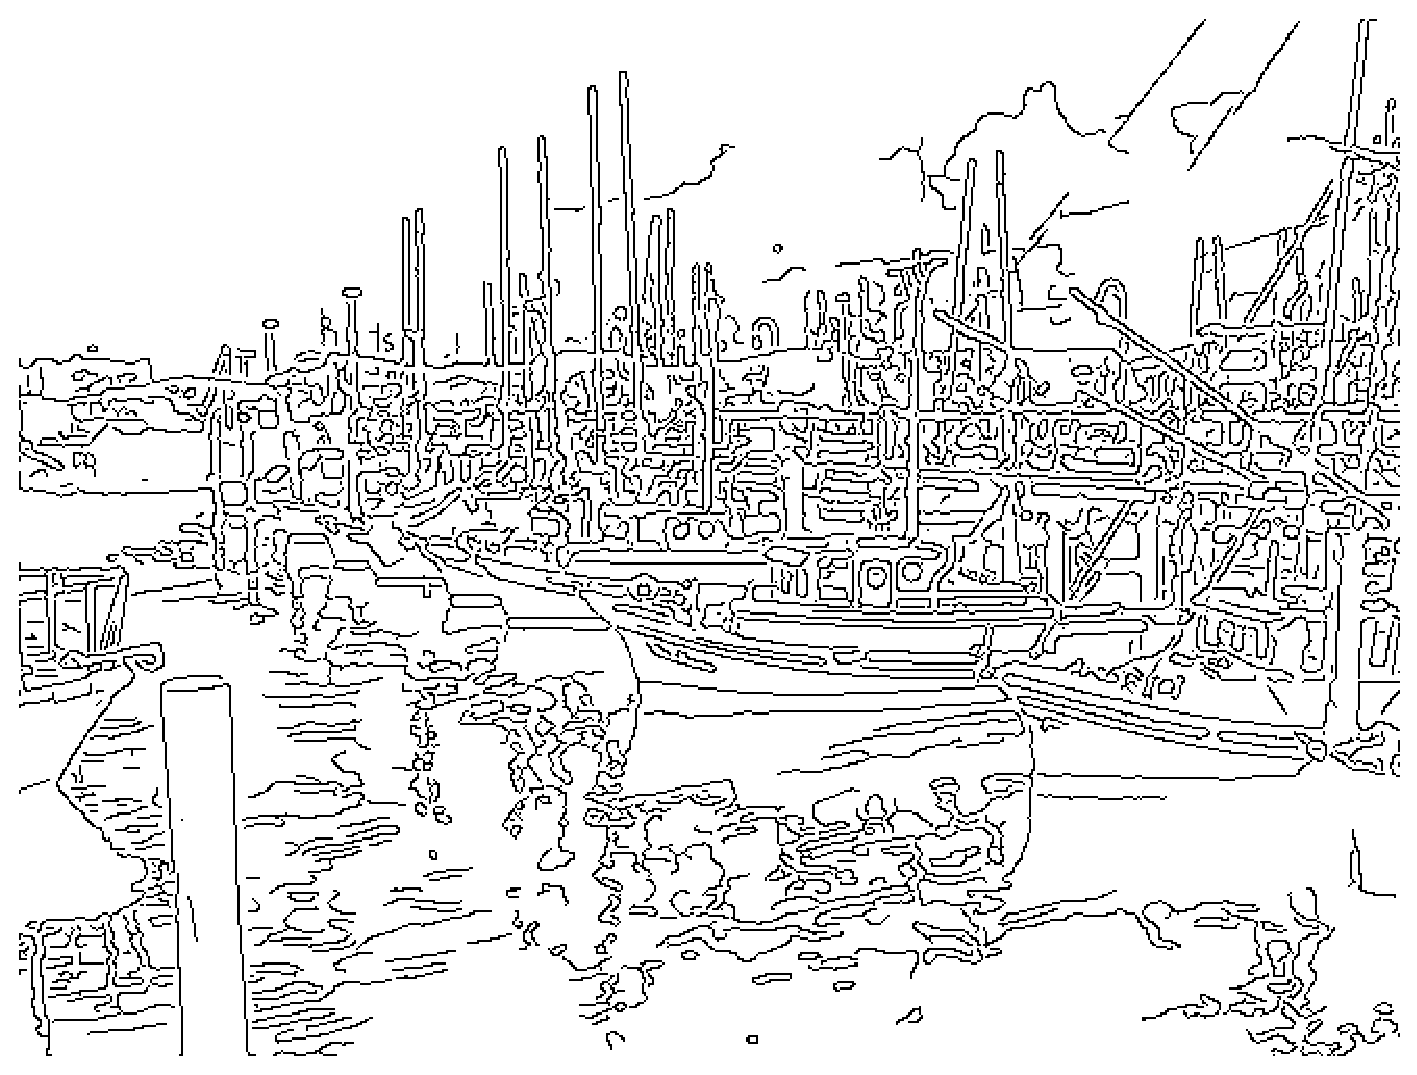
\includegraphics[width=2.4in]{pictures/boat_in_sf/canny.eps}}
	}
	\caption{Boats at the Bay}\label{fig:Compare4}
\end{figure}
The current implementation of our Adaptive-DoG filter is not optimized for performance yet. Currently, it runs significantly slower than DoG and FDoG, due to the image segmentation step. Our implementation of polarity calculation requires $1344 ms$ to perfoms on image with $750*500$ dimension with size of neigborhood at $20*20$ pixels. The Adaptive-DoG filter itself runs for $3390 ms$ on the same image. The total run time for this technique is $7797 ms$. This number is significantly higher DoG, which only requires $3859 ms$, and also FDoG, which only requires $4578 ms$. The main problem from our implementation is that we still apply both DoG and FDoG filters, in which both output will be selectively chosen based on image segment. Further improvement of this implementation is required to make the program run faster and more efficient.

\chapter{Conclusion}
Our Adaptive-DoG technique, regardless the performance in term of speed, is able to produce better results when compared to DoG and FDoG in many different variaty of images in our experiment. The lines appear to be more continuous than lines in DoG images, and the details in coarse texture is better maintain than FDoG images.

Although the output is relatively better in some cases, the results of Adaptive-DoG may never exceed the results of neither DoG nor FDoG in some specific cases. For input image that only contains lines without any coarse texture, the results of Adaptive-DoG will, at best, be the same with FDoG, while for input image with coarse texture only, the results will never exceed DoG.

Another note from experiment experiment that we need mention is the performance in term of runtime. Our experiment shows that the performance of the filter is relatively lower than both preceding filters. Nevertheles, with more code optimization and tweaking, some improvements are possible to be achieved.

Possible future improvement for Adaptive-DoG is by iterating the filters to prouduce more solid shape for both lines and textures. The same polarity map may be use on the next iteration, but generating new polarity map might also produce better results.

%\chapter{Future Implementation}
%\section{Speed-up of Image Segmentation}

\bibliography{main} 
\bibliographystyle{plain} 
